\begin{flushleft}
Dobbiamo studiare il minimo della funzione a più variabili $f(x_1,x_2)=x_1^4+x_1\cdot(x_1+x_2)+(1+x_2)^2$, per fare questo è necessario trovare i punti stazionari del gradiente della funzione f:
\[
\nabla f \cdot \begin{pmatrix} x_1 \\\ x_2 \end{pmatrix} = \underline{0}
\]
Con $\nabla f$ calcolato come segue:
\[
\nabla f = \begin{pmatrix} \frac{\partial f}{\partial x_1} \\\ \frac{\partial f}{\partial x_2} \end{pmatrix} = \begin{pmatrix} 4\cdot x_1^3+2\cdot x_1 + x_2 \\\ x_1+2\cdot(1+x_2)\end{pmatrix}
\]
A questo punto è possibile usufruire della function MatLab nonLinearNewton implementata precedentemente per trovare la soluzione di questo sistema lineare. Per poterla usare è però necessario trovare la matrice jacobiana di $\nabla f$ (che non è altro che la matrice hessiana di f):
\[
J\nabla f = \begin{pmatrix} \frac{\partial (\nabla f_1)}{\partial x_1} & \frac{\partial (\nabla f_1)}{\partial x_2}  \\\ \frac{\partial (\nabla f_2)}{\partial x_1} & \frac{\partial (\nabla f_2)}{\partial x_2} \end{pmatrix} = \begin{pmatrix} 12x_1^2+2 & 1  \\\ 1 & 2 \end{pmatrix}
\]
Abbiamo quindi scritto lo script:
\lstinputlisting[language=Matlab]{cap_3/es21/es21.m}
che restituisce in output il risultato:
\begin{figure}[H]
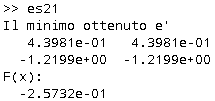
\includegraphics[left, width=300px]{cap_3/es21/es321}
\end{figure}
$\underline{x^*} = \begin{pmatrix} 4.3981e-01 & -1.2199e+00 \end{pmatrix}$ rappresenta quindi il punto di minimo della funzione $f(x_1,x_2)=x_1^4+x_1\cdot(x_1+x_2)+(1+x_2)^2$. Andando a sostituire i valori si ottiene:
\[
f(\underline{x^*}) = (0,43981)^4+(0,43981)\cdot(0,43981-1,2199)+(1-1,2199)^2 = -0.25732
\]
\end{flushleft}